\documentclass{article}
\usepackage{graphicx,fancyhdr,amsmath,amssymb,amsthm,subfig,url,hyperref}
\usepackage[margin=1in]{geometry}

\newcommand{\studentname}{Francois Chaubard and Colin Mayer}
\newcommand{\suid}{fchaubard, cmayer}
\newcommand{\assignment}{Programming Assignment 1}

\renewcommand{\theenumi}{\bf \Alph{enumi}}


\fancypagestyle{plain}{}
\pagestyle{fancy}
\fancyhf{}
\fancyhead[RO,LE]{\sffamily\bfseries\large Stanford University}
\fancyhead[LO,RE]{\sffamily\bfseries\large CS 224N: Natural Language Processing}
\fancyfoot[LO,RE]{\sffamily\bfseries\large \studentname: \suid}
\fancyfoot[RO,LE]{\sffamily\bfseries\thepage}
\renewcommand{\headrulewidth}{1pt}
\renewcommand{\footrulewidth}{1pt}

\graphicspath{{figures/}}

%-------------------------------- Title ----------------------------------

\title{CS224N \assignment}
\author{\studentname \qquad SUNet ID: \suid}

%--------------------------------- Text ----------------------------------

\begin{document}
\maketitle

\section*{Word Alignment Models}

The first two models studied here, take a frequentist approach to word translations. We count the number of times words occur in the target and source languages, and also the source/target pairs of words over a set of parallel sentences. In the PMI model, we ignore the alignments of words and only concern ourselves with word for word translation “counts”. This only requires one iteration over the test set to gather the counts. A fairly weak model that is losing a lot of the color of the dataset.

In IBM Model 1, we learn soft assignment word translation probabilities via variable assignments taken from previously estimated word translation probabilities. Here we need to establish a convergence criterion since this iterative algorithm could possibly run forever. Since this EM problem is convex in the soft assignments, we know that there is an optimal word translation probability that we are approaching. Thus, our chosen convergence criteria is, when the change in our source/target soft assignments from one EM iteration to the next is below L2 distance of 0.5, we say we are close enough to the optimal solution. 

Finally, for IBM Model 2, we no longer assume uniform probability of alignments in each of the sentence pairs, but instead treat these alignment probabilities as latent variables to be found. We look at the position of a target word, the length of each of the pair of sentences, and suggest that this “distortion” distribution has meaningful statistical inference, despite being word agnostic. We learn these soft assignments in a very similar approach as in the word pairing distributions, and iteratively converge onto a solution. In such a Bayesian manner, we score highly alignments of words that have both, a language to language disposition for such a word reordering as well as a specific word for a specific word translation. In plainer english, we take into account the position of the word. 

A hurdle to overcome now is that of convergence, since the problem is no longer convex having added a non-linear product (multiplication of the word translation probabilities and the assignment distortion probabilities). So what makes for a good convergence criteria now since we are not necessarily approaching a global optima? This one is less obvious so we perform both a limited “for” loop operation ending after 50 iterations and also calculate change in the distributions in the same way except this time we do it for both the distortion probabilities and the translation probabilities, and when the sum of these two is less than 0.04, we declare convergence.

\section*{Word Alignment Results}
All values shown are the Alignment Error Rate (AER)
\begin{center}
\captionof{table}{Dev Set} \label{tab:title} 
\def\arraystretch{1.5}
\begin{tabular} {c|c|c|c}
 &French&Hindi&Chinese \\
\hline
PMI&0.7608&0.8760&0.8626 \\
IBM1&0.3534&0.5852&0.5869 \\
IBM2&0.2913&& \\
\end{tabular}


\captionof{table}{Test Set} \label{tab:title} 
\begin{tabular} {c|c|c|c}
 &French&Hindi&Chinese \\
\hline
PMI&0.7505&0.8458&0.8410 \\
IBM1&0.3494&0.5810&0.5893 \\
IBM2&0.3024&0.5858&0.5605 \\
\end{tabular}
\end{center}
\section*{MT Feature Engineering}

After building the Phrasal installation and running the baseline feature set, we looked through the phrase table for possible indicator features. One interesting metric was the relationship between the number of words in the source phrase and the number of words in the target phrase. For languages with similar syntax and common lineage like French and English it seemed that equivalent phrases should contain similar numbers of words. As a (semi)-bilingual team, study of the phrase tables found that for many of the more accurate phrase pairs the French phrase contained 0 or 1 additional words than the English phrase. This was particularly common for short phrases with verb negation or series of articles. For example the following phrase pairs:
\begin{center}
\begin{tabular}{l l c c}
French & English & French Size & English Size \\
le jugement n' est pas & the ruling is not & 5 & 4 \\
ou des radicaux & or radicals & 3 & 2 \\
nous ne pouvons pas & we can not & 4 & 3 \\
une fois par semaine & once a week  & 4 & 3 \\
\end{tabular}
\end{center}
To capture this behavior we designed a feature that fired whenever a French phrase (length of 3 words or more) was paired with an English phrase with the same length or one fewer word. This feature did not have a significant effect on the result metrics, gaining a weight of 0.07 and a BLEU score of 14.993 compared to 14.756  for the baseline. Qualitative analysis of the translation found that our feature mostly affected articles and other common words explaining its negligible impact on the BLEU score. However, we saw in many cases that target sentences had a more natural sounding flow for series of articles. Because the feature favored target phrases of equal or lesser length, one would think that it would produce translations with shorter English phrases. The opposite turned out to be true, as the MT system is known to favor shorter phrases in general, the same length or one word less feature pulled the system towards longer target phrases. Improvements in the natural sound of sentences were most likely due to this behavior. The examples highlight some of the improvements over the baseline translation our feature offered.

\begin{description}

\item[Phrase Pair 1]
\item[Baseline] there are many examples of various appearances and i am pleased that i all week to sort all the information received .

\item[With Feature] there are many examples of various appearances and i am pleased that i have a whole week to sort all the information received .

\item[Phrase Pair 2]
\item[Baseline] the two teams had difficulty up combinations and concentrating primarily around the centre line.

\item[With Feature] the two teams had difficulty up combinations and the game focused primarily around the centre line .
\end{description}

\section*{Error Analysis}

As expected the naive PMI model performs poorly in all languages. The IBM1 model performs significantly better than PMI for French-English alignment, AER of 0.35 vs. AER 0.76, and French-English error rates are further improved with the IBM2 Model AER of 0.30. This is most likely because French and English have common etymology and often have consistent sentence alignment patterns. The error rates for Hindi and Chinese are higher for both models and we see little to no improvement between IBM1 and IBM2. Both models show poor recall for Hindi and Chinese, meaning the models had difficulty determining word pairs, regardless of alignment, which would explain why incorporating the word alignment model in IBM2 has minimal effect on the results. In the case of Hindi-English alignment one reason for the poor recall could be that Hindi contains significantly more word morphology, of both nouns and verbs, than English.

One factor that contributed to poor performance with the Hindi-English alignment was the limited size of the Hindi training set. The Hindi training set only had 3441 sentence pairs, compared to the 10,000 sentence pairs used for French and Chinese. While more data does not guarantee improved performance, the difference between training sets of 3,500 and 10,000 pairs can be significant. For example if the French-English training set is limited to 3,500 pairs the AER increases by almost from 20\% from 0.35 to 0.41.

Another reason that error rates are significantly higher in Hindi and Chinese is in part due to our one to many mappings for the Null word. Since there are no articles in Chinese as there are in English, articles such as “the”, “a”, and “an” are all being mapped to the Null word so the translation score confuses these 3 consistently. A better language model could rectify these differences. 

Examination of the alignment tables finds that both IBM models perform very well for sentence pairs with strong one-to-one word correlation and diagonal alignments. In sentence pairs that have multiple one-to-many alignment options the model performance degrades quickly and it often aligns many target words to one incorrect source word
\begin{center}
\begin{figure}[h]
\caption{Example Alignment Table}
\centering
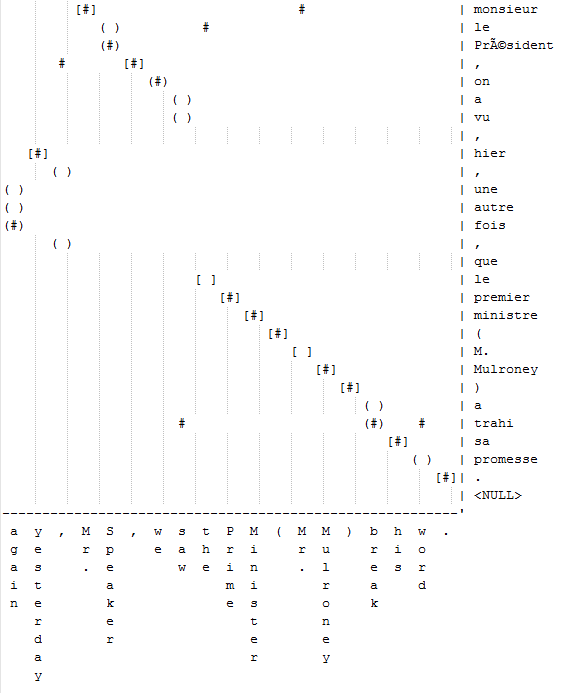
\includegraphics[width=0.5\textwidth]{alignment_table}
\end{figure}
\end{center}
\section*{IBM Model 2 Optimization}

\end{document}
